\documentclass{fizykalab}

% Ustawienia do tabelki

\wydzial{WI}
\autorjeden{Piotr Karamon}
\autordwa{Hubert Kasprzycki}
\rok{2}
\grupa{12}
\zespol{5}
\temat{Kondensatory}
\nrcwiczenia{33}
\datawykonania{24.10.2023}
\dataoddaniajeden{31.10.2023}
\zwrotdopoprawy{}
\dataoddaniadwa{}
\datazaliczenia{}

\usepackage{amsmath}
\usepackage{amsfonts}
\usepackage{parskip}

\newenvironment{conditions}[1][gdzie:]
  {#1 \begin{tabular}[t]{>{$}l<{$} @{${} - {}$} l}}
  {\end{tabular}\\[\belowdisplayskip]}

% \renewcommand{\arraystretch}{1.5}
\newcolumntype{L}[1]{>{\raggedright\let\newline\\\arraybackslash\hspace{0pt}}m{#1}}
\newcolumntype{C}[1]{>{\centering\let\newline\\\arraybackslash\hspace{0pt}}m{#1}}
\newcolumntype{R}[1]{>{\raggedleft\let\newline\\\arraybackslash\hspace{0pt}}m{#1}}

\usepackage[left=1.75cm, right=2cm, top=3cm]{geometry}
\usepackage[labelfont=bf]{caption}

\newcommand{\nm}{\ensuremath{\text{nm}}}
\newcommand{\mm}{\ensuremath{\text{mm}}}
\newcommand{\m}{\ensuremath{\text{m}}}
\newcommand{\um}{\ensuremath{\mu \text{m}}}
\newcommand{\ju}{\ensuremath{\text{j.u.}}}
\newcommand{\cde}{\ensuremath{(Cd)_\text{extr}}}
\newcommand{\mmpF}{\ensuremath{\text{mm}\cdot\text{pF}}}
\newcommand{\Fm}{\ensuremath{\frac{\text{F}}{\text{m}}}}


\usepackage{natbib}
\usepackage{url}
\begin{filecontents*}{test.bib}
@MISC{elportal-zlacze,
    author = {Michał Kurzela},
    title = {Dioda prostownicza - charakterystyka, oznaczenia, budowa},
    year = {2022},
    note = {[\url{https://elportal.pl/i/2022/09/06/12517-cfe4-1600x0_089-04.jpg}; odwiedzona  14.10.2023]},
    url = {https://elportal.pl/i/2022/09/06/12517-cfe4-1600x0_089-04.jpg}
}
\end{filecontents*}

\begin{document}

\maketitle

\section{Cel ćwiczenia}
Pomiar pojemności kondensatorów powietrznych i z warstwą
dielektryka w celu wyznaczenia stałej elektrycznej 
$\varepsilon_0$ (przenikalności dielektrycznej próżni)
i przenikalności względnych $\varepsilon_r$ różnych materiałów.

\section{Wstęp teoretyczny}
\subsection{Podstawy kondensatorów oraz wyznaczanie stałej elektrycznej}
Kondensator jest układem przewodników oddzielonych warstwą izolatora. 
Przez pojemność kondensatora $C$ 
rozumiemy stosunek ładunku $Q$ do napięcia między okładkami $U$
czyli $C = \frac{Q}{C}$

Popularny, acz uproszczony wzór na pojemność kondensatora płaskiego
\begin{equation}
    \label{eq:C_basic}
    C = \frac{\varepsilon_0 \varepsilon_r S}{d}
\end{equation}

Wartości $\varepsilon_0$ nie możemy wyznaczać wprost z powyższego wzoru
z dwóch powodów.
\begin{itemize}
    \item Po pierwsze krążki określające odległość $d$ między płytami wykonane
    są z materiału o przenikalności dielektrycznej $\varepsilon_r$
    znacznie większej od jedności, co powoduje powiększenie całkowitej
    pojemności kondensatora.
    \item Drugi powód to istnienie pola rozproszonego.
    Z praw elektrostatyki wynika, że poza brzegami
    kondensatora istnieje niejednorodne (o zakrzywionych liniach sił)
    pole elektryczne, nazywane
    polem rozproszonym.
    Pole rozproszone powoduje dodatkowy wzrost pojemności
    kondensatora.
\end{itemize}

\begin{figure}[H]
    \centering
    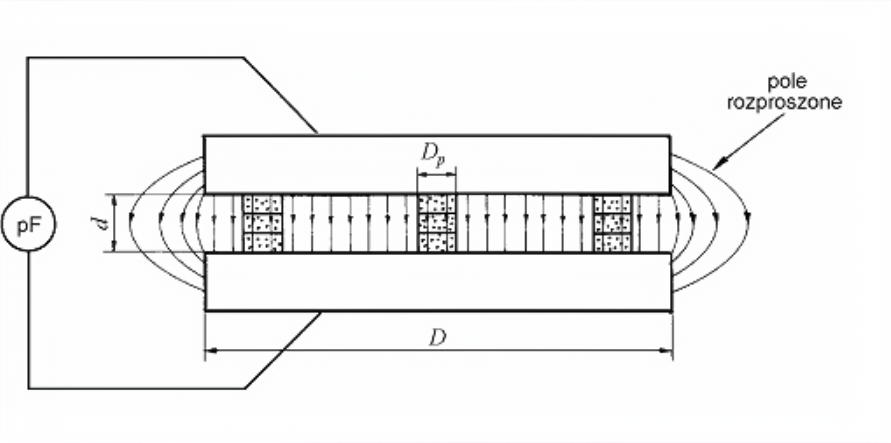
\includegraphics[width=0.5\linewidth]{download.png}
    \caption{Powietrzny kondensator płaski z trzema słupkami dielektryka}
    \label{fig:kondensator}
\end{figure}

W naszym eksperymencie przybliżeniem kondensatora próżniowego jest kondensator
powietrzny rysunek \ref{fig:kondensator}. Okładkami kondensatora są kołowe płyty metalowe.
Określoną odległość
między płytami uzyskuje się przez umieszczenie w trzech miejscach 
stosu izolujących krążków.
Do pomiaru pojemności kondensatora stosujemy cyfrowy miernik pojemności.

Kondensator nasz potraktować można jako równoległe połączenie kondensatora
z dielektrykiem o przenikalności względnej $\varepsilon_r$ i łącznej 
powierzchni okładek równej $3S_p$ (gdzie
$S_p$ jest powierzchnią jednego krążka) oraz kondensatora próżniowego,
o powierzchni okładek równej $S - 3S_p$.

Pojemność całkowita wynosi:
\begin{equation*}
    C = \frac{\varepsilon_0(S - 3S_p)}{d} + 
        \frac{\varepsilon_0 \varepsilon_r 3S_p}{d} 
\end{equation*}

Z powyższego wzoru wartość $\varepsilon_0$  obliczamy jako
\begin{equation}
    \label{eq:e0}
    \varepsilon_0  = \frac{Cd}{S + 3(\varepsilon_r - 1) S_p}
\end{equation}

Ten wzór jednak nadal nie uwzględnia 
pola rozproszonego.
W naszym ćwiczeniu zastosujemy doświadczalny sposób eliminacji wpływu pola rozproszonego.
Efektywna objętość  pola rozproszonego jest rzędu $2 \pi r d^2$
, gdyż pole to zajmuje z grubsza pas
o wysokości i szerokości rzędu $d$ wokół obwodu kołowych płyt kondensatora. Natomiast
objętość pola jednorodnego wewnątrz kondensatora wynosi $\pi r^2 d$.
Względny udział pola
rozproszonego, będący stosunkiem tych objętości, wynosi $2d/r$, czyli że maleje do zera w
granicy $d \to 0$. 


Wykonamy zatem serię pomiarów pojemności $C$ dla różnych wartości $d$, a następnie
wykres iloczynu $Cd$ w funkcji odległości okładek $d$.
Przez uzyskane punkty wykresu przeprowadzamy analitycznie gładką krzywą
i ekstrapolujemy, czyli przedłużamy do wartości $d = 0$. Współrzędną punktu przecięcia
krzywej $Cd = f(d)$ z osią pionową nazywamy ekstrapolowaną wartością iloczynu $\cde$ .
Wartość $\cde$ podstawiamy do licznika wzoru (\ref{eq:e0}) by 
uzyskać poprawną wartość $\varepsilon_0$.
Ponadto powierzchnię okładki kondensatora $S$ i przekładki $S_p$ obliczamy na podstawie
zmierzonych średnic $D$ i $D_p$, czyli $S = \pi \frac{D^2}{4}$ oraz $S = \pi \frac{D_p^2}{4}$
W ten sposób otrzymujemy wzór końcowy na $\varepsilon_0$.

\begin{equation}
    \label{eq:e0_final}
    \varepsilon_0 = \frac{4}{\pi}
                    \frac{\cde}{D^2 + 3(\varepsilon_r -1) D_p^2}
\end{equation}
\subsection{Obliczanie prędkości światła}

Aby obliczyć prędkość światła w próżni wykorzystamy 
wcześniej obliczoną stałą $\varepsilon_0$ oraz wzór
\begin{equation}
    \label{eq:light}
    c = \frac{1}{\sqrt{\varepsilon_0 \mu_0}}
\end{equation}

Będziemy do tego potrzebować jeszcze jednej stałej $\mu_0$
której wartość wynosi
\begin{equation*}
    \mu = 4\pi \cdot 10 ^{-7} \frac{\text{Vs}}{\text{Am}}
\end{equation*}

\subsection{Pomiar przenikalności względnej dielektryków}
Wartość $\varepsilon_r$
dielektryków stałych  wyznaczyć można przez pomiar pojemności
kondensatora płaskiego z okładkami oddzielonymi cienką płytą z badanego materiału.
Korzystamy ze wzoru (\ref{eq:C_basic}),
poprawki na pole rozproszone nie będziemy uwzględniać.

\subsection{Kabel koncentryczny}
Obok kondensatora płaskiego przykładem obiektu o określonej pojemności jest kabel
koncentryczny. Można go traktować jako kondensator cylindryczny,
którego jedną okładką jest środkowy drut, drugą – miedziany oplot.
Pojemność kondensatora cylindrycznego wyraża wzór

\begin{equation}
    \label{eq:kabel}
    C = \frac{2 \pi \varepsilon_0 \varepsilon_r l}
             {\ln \frac{R}{r}}
\end{equation}
\begin{conditions}
    $R$ & promień zewnętrzny \\
    $r$ & promień wewnętrzny \\
    $l$ & długość kabla \\
\end{conditions}

\section{Aparatura pomiarowa}
Układ pomiarowy składa się z kondensatora z 
rysunku $\ref{fig:kondensator}$ oraz z cyfrowego 
miernika pojemności.
Kondensator składa się z dwóch
kołowych płyt metalowych o płaskiej powierzchni oraz z przekładek
wytoczonych z płyty pleksiglasowej.
Do pomiarów geometrycznych używamy
przymiaru milimetrowego (linijka) i śruby mikrometrycznej. 


\section{Przebieg doświadczenia}

Na początku eksperymentu, konieczne było uruchomienie miernika LCR i ustawienie zakresu na 200 pF. W następnym etapie, dokonaliśmy pomiarów grubości przekładek z pleksiglasu. Umieściliśmy je na dolnej okładce kondensatora i położyliśmy na nich okładkę górną. Następnie przeprowadziliśmy pomiar pojemności kondensatora. Kolejno dokonaliśmy pomiaru pojemności kondensatora dla 2, 3, 4, 5 przekładek oraz ponownie dla jednej przekładki. Następnie umieściliśmy między okładkami kondensatora płyty wykonane z drewna, pleksiglasu i PCV, wcześniej zmierzając ich grubości. Kolejnym obiektem poddanym badaniu był kabel koncentryczny. Dokonaliśmy pomiaru jego długości, średnicy wewnętrznej i zewnętrznej oraz pojemności. 

\section{Wyniki pomiarów}

\subsection{Kondensator płaski}

\begin{table}[H]
    \centering
    % \begin{tabular}{|c|c|c|c|c|c|c|}
    \caption{Pomiar pojemności kondensatora w funkcji odległości elektrod}
    \begin{tabular}{|c|C{2cm}|C{2cm}|C{2cm}|C{3cm}|C{2cm}|C{2cm}|}
        \hline
        przekładki & $d_1$ [\mm] & $d_2$ [\mm] & $d_3$ [\mm] & $d=\frac{d_1 + d_2 + d_3}{3}$ [\mm] & $C$ [pF] & $Cd$ [$\mm\cdot\text{pF}$] \\ \hline
        1 & 4.35 & 4.32 & 4.36 & 4.34 & 118.4 & 514.25 \\ \hline
        2 & 7.04 & 6.81 & 6.8 & 6.88 & 71.2 & 490.09 \\ \hline
        3 & 10.93 & 10.65 & 10.66 & 10.75 & 48.3 & 519.06 \\ \hline
        5 & 14.75 & 14.5 & 14.54 & 14.6 & 37.7 & 550.29 \\ \hline
        4 & 16.6 & 16.65 & 16.36 & 16.54 & 31.3 & 517.6 \\ \hline
        1 & 3.63 & 3.85 & 3.63 & 3.7 & 121.2 & 448.84 \\ \hline
    \end{tabular}
    \label{tab:capacity-measure-dist}
\end{table}

Średnica kondensatora: 24 cm \\
Średnica przekładki: 20.05 \mm

\subsection{Kondensator płaski z dielektrykami}
\begin{table}[H]
    \centering
    \caption{Pomiar pojemności kondensatora w zależności od użytek materiału }
    \begin{tabular}{|C{3cm}|C{3cm}|C{3cm}|}
        \hline
        materiał & $d$ [mm] & $C$ [pF]\\ \hline
        drewno & 9.71 & 201\\ \hline
        PCV & 3.11 & 374\\ \hline
        pleksiglas & 3.9 & 311\\ \hline
    \end{tabular}
    \label{tab:capacity-measure-material}
\end{table}

\subsection{Kabel koncentryczny}

Średnica zewnętrzna $2R$ = 5 mm \\
Średnica wewnętrzna $2r$ = 1.19 mm \\
Długość $l$ = 65.5 cm \\
Pojemność kabla $C$ = 32.5 pF \\

\section{Opracowanie wyników}
\subsection{Obliczanie stałej elektrycznej i prędkości światła w próżni}
Aby obliczyć $\cde$ rysujemy wykres rysujemy wykres $Cd = f(d)$ 
a następnie dopasowujemy do niego krzywą $y = ax^2 + bx + c$.
\begin{figure}[H]
    \centering
    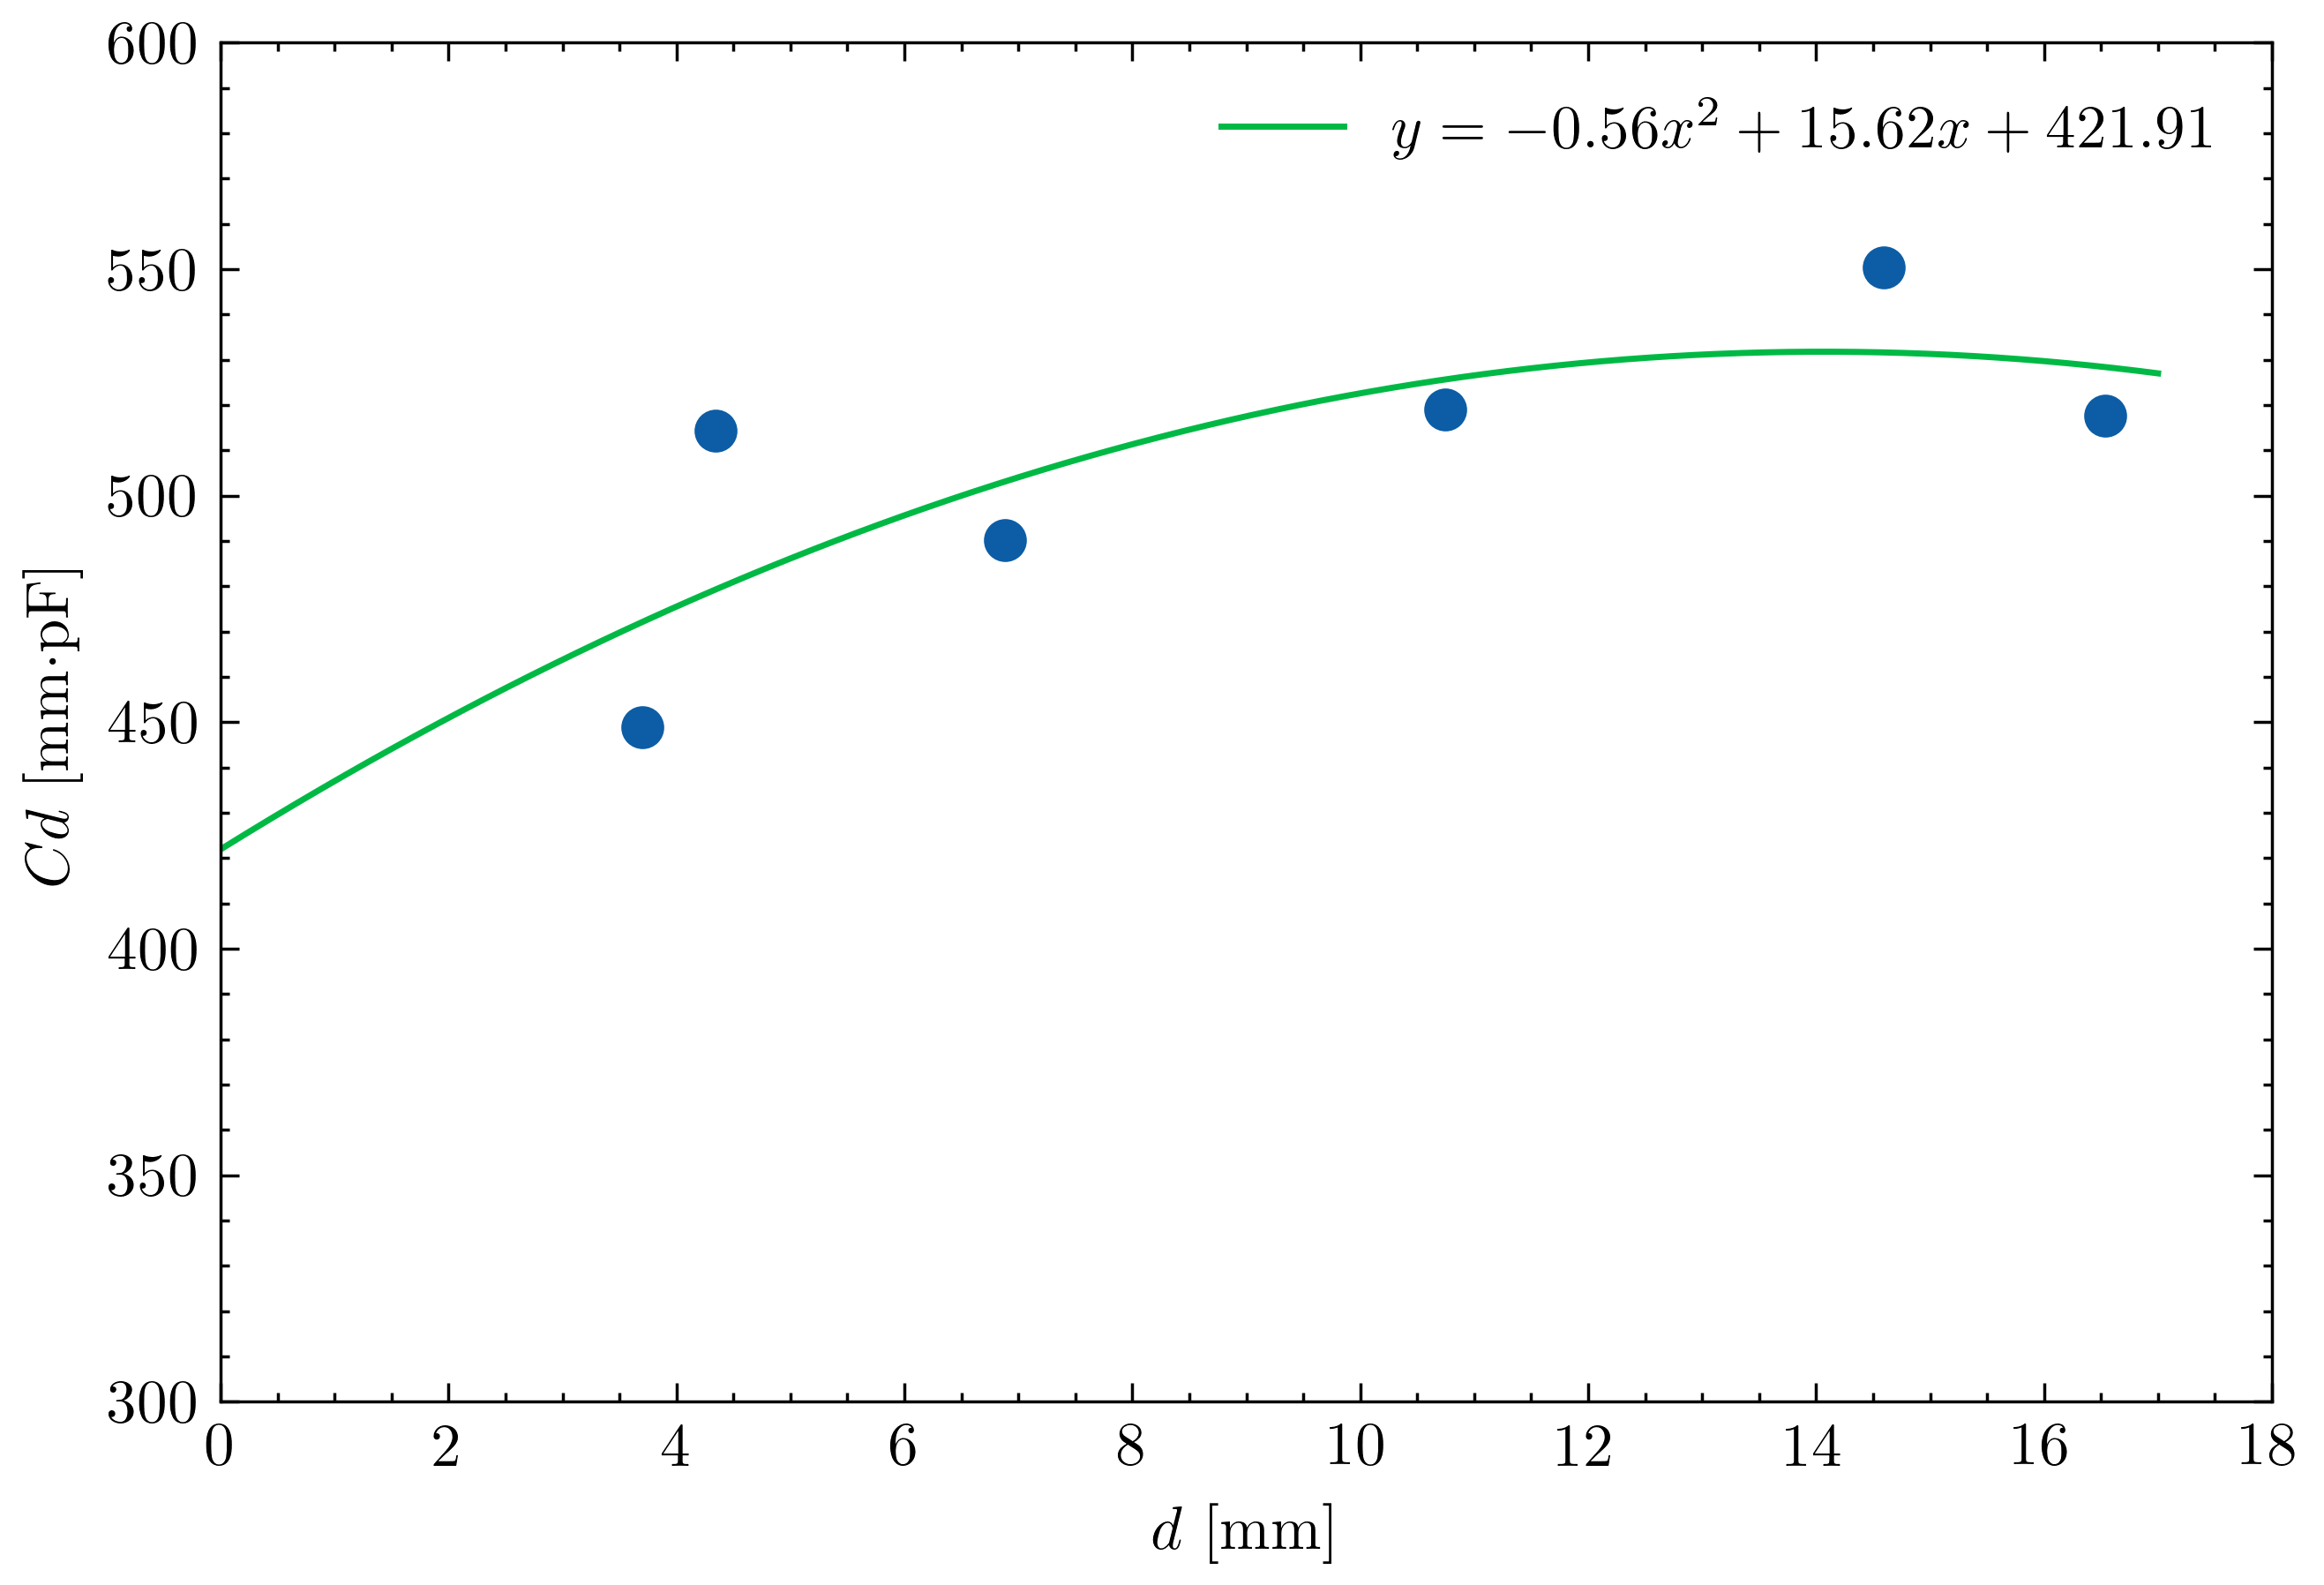
\includegraphics[width=0.75\linewidth]{wykres.png}
    \caption{Wykres $Cd = f(d)$ z dopasowaną gładką krzywą.}
\end{figure}

Z wykresu oraz obliczeń programu który dopasował krzywą wynika

\begin{align}
    u(\cde) &= 63 \mmpF \\
    \cde &= 421.91 \mmpF = 422 \mmpF
\end{align}

Aby obliczyć $\varepsilon_0$ wykorzystamy wzór (\ref{eq:e0_final}),
natomiast by obliczyć niepewność naszego wyniku wykorzystamy wzór w którym 
pominiemy wyraz poprawkowy $3(\varepsilon_r - 1) D_p^2$, czyli 
wzór:
\begin{equation*}
    \varepsilon_0 = \frac{4}{\pi} \frac{\cde}{D^2}
\end{equation*}

Zatem stosujemy prawno przenoszenia niepewności w wyniku czego otrzymujemy:
\begin{align}
\begin{split}
    u(\varepsilon_0) &= \sqrt{
        \left[ \frac{\partial \varepsilon_0}{\partial \cde} \cdot u(\cde) \right]^2 + 
        \left[ \frac{\partial \varepsilon_0}{\partial \cde} \cdot u(D)\right]^2
    } =\\ &=
    \sqrt{ 
         \left[ \frac{4}{\pi D^2} \cdot u(\cde) \right]^2+
         \left[ \frac{8 \cde}{\pi D^3} \cdot u(D) \right]^2
    } = \\ &=
    \sqrt {
         \left[ \frac{4}{\pi (240 \mm)^2} \cdot 63 \mmpF \right]^2 +
         \left[ \frac{8 \cdot422\mmpF}{\pi (240 \mm)^3} \cdot 1\mm \right]^2 
    } = \\ &= 1.381 \cdot 10^{-12} \Fm =  1.4 \cdot 10^{-12} \Fm
\end{split}
\end{align}

Przekładki były wykonane z pleksiglasu zatem użyjemy $\varepsilon_r = 2,6$.
\begin{align}
\begin{split}
    \varepsilon_0 = \frac{4}{\pi}
                    \frac{\cde}{D^2 + 3(\varepsilon_r -1) D_p^2} = 
                    \frac{4}{\pi}
                    \frac{422 \mmpF}{(240 \mm)^2 + 3(2.6 -1) (20.05 \mm)^2} = 9.024 \cdot 10^{-12}\Fm
\end{split}
\end{align}

Niepewność rozszerzona $U(\varepsilon_0)$ jest równa $U(\varepsilon_0) = 2\cdot u(\varepsilon_0) = 2,8 \Fm$
Ostatecznie możemy zapisać:
\begin{equation}
    \varepsilon_0 = 9.024 \cdot 10^{-12} \Fm \pm 2.8 \cdot 10^{-12} \Fm
\end{equation}

Wyliczona przez nas wartość jest zgodna z wartością tabelaryczną wynoszącą
$\varepsilon_0 = 8.542 \cdot 10^{-12} \Fm $. Trzeba jednakże przyznać, że
uzyskana przez nas niepewność jest bardzo duża. Może to być wynikiem
błędów ludzkich takich jak niestaranność w mierzeniu grubości przekładek
lub niedokładne ułożenie płyt
kondensatora jedna nad drugą lub przekładek.
Możliwe również, że część winy za dużą niepewności stoi po 
stronie sprzętu oraz otoczenia.
Miernika nie byliśmy w stanie wyzerować, był
zasilany bateriami, które mogły już nie być 
w najlepszej kondycji. Tutaj również należy 
wspomnieć o tym, iż mamy  tutaj do czynienia
z kondensatorem powietrznym, który jest
tylko przybliżeniem kondensatora próżniowego.

Aby wyliczyć prędkość światła skorzystamy ze wzoru (\ref{eq:light}), 
wynika z niego, że $c$ jest funkcją jednej zmiennej $\varepsilon_0$
aby obliczyć niepewność pomiaru skorzystamy z prawa przenoszenia niepewności.

\begin{align*}
    u(c) &= \sqrt{ \left( \frac{\partial c}{\partial \varepsilon_0}
                         \cdot u(\varepsilon_0) \right)^2}
    = \left| \frac{u(\varepsilon_0)}{\sqrt{\mu_0} \cdot 2\varepsilon_0^{\frac{3}{2}}} \right| 
    = \left| \frac{1.381 \cdot 10^{-12} \Fm}
    {
    \sqrt{4\pi \cdot 10^{-7} \frac{\text{Vs}}{\text{Am}}}
    \cdot
    2 \cdot \left(  9.024 \cdot 10^{-12} \Fm \right)^ {\frac{3}{2}}
    }  \right| = 22722709 \frac{\text{m}}{\text{s}} = 23000000 \frac{\text{m}}{\text{s}} \\
    c &= \frac{1}{\sqrt{\varepsilon_0 \mu_0}} = 
    \frac{1}{\sqrt{9.042 \cdot 10^{-12} \Fm \cdot 4 \pi \cdot 10^{-7} \frac{\text{Vs}}{\text{Am}}} } = 
    296662612\frac{\text{m}}{\text{s}}
\end{align*}

Zatem niepewność rozszerzona $U(c)$ jest równa 
$U(c) = 2\cdot u(c) = 46 000 000 \frac{\text{m}}{\text{s}}$ 

Ostatecznie możemy zapisać
\begin{equation*}
    c = 296662612\frac{\text{m}}{\text{s}} \pm 4.6 \cdot 10^7 \frac{\text{m}}{\text{s}}
\end{equation*}
Wyliczona przez nas wartość prędkości światła jest zgodna z wartością tabelaryczną.
Uzyskana niepewność, jest nie ma co się oszukiwać podobnie jak w przypadku $u(\varepsilon_0)$,
bardzo duża. Zapewne z powodu tych samych powodów, o których pisaliśmy 
wyżej przy obliczaniu $u(\varepsilon_0)$.


\subsection{Obliczanie przenikalności względnej materiałów}

Aby obliczyć $\varepsilon_r$ skorzystamy ze wzoru
(\ref{eq:C_basic}) odpowiednio go przekształcając
w wyniku czego otrzymujemy.

\begin{equation}
    \varepsilon_r = \frac{Cd}{\varepsilon_0 S }
\end{equation}

Zatem dla drewna:
\begin{equation*}
    \varepsilon_r = \frac{Cd}{\varepsilon_0 S } = 
    \frac{201 \text{pF} \cdot 0.00971 \mm}
    {8.8542 \cdot 10^{-12} \Fm \cdot \pi (\frac{0.240 \text{m}}{2})^2 } = 4.873
\end{equation*}
Dla drewna wartość $\varepsilon_r$ powinna się mieścić w przedziale $(2, 7)$
wyliczona przez nas wartość mieści się w tym przedziale.

Dla PCV:
\begin{equation*}
    \varepsilon_r = \frac{Cd}{\varepsilon_0 S } = 
    \frac{374 \text{pF} \cdot 0.00311 \mm}
    {8.8542 \cdot 10^{-12} \Fm \cdot \pi
    (\frac{0.240 \text{m}}{2})^2 } = 2.904
\end{equation*}
Wartość tabelaryczna dla PCV jest równa $2.8$, wyliczona
przez nas wartość jest do niej zbliżona.

Dla pleksiglasu:
\begin{equation*}
    \varepsilon_r = \frac{Cd}{\varepsilon_0 S } = 
    \frac{311 \text{pF} \cdot 0.00390 \mm}
    {8.8542 \cdot 10^{-12} \Fm \cdot \pi
    (\frac{0.240 \text{m}}{2})^2 } = 3.029
\end{equation*}
Wartość tabelaryczna dla pleksiglasu jest równa $2.6$ 
wyliczona przez nas wartość jest porównywalna,
lecz widocznie wyższa.


\subsection{Przenikalność względna kabla koncentrycznego}
Aby obliczyć $\varepsilon_r$ dla kabla 
przekształcamy wzór (\ref{eq:kabel}) otrzymując

\begin{equation*}
    \varepsilon_r = \frac{C \ln \frac{R}{r}}{2 \pi \varepsilon_0 l}
\end{equation*}
Następnie podstawiamy dane:

\begin{equation*}
\varepsilon_r = \frac{32.5 \text{pF}
\ln \frac{2.5 \mm}{0.595 \mm}}{2 \pi  \cdot 8.8542 \cdot 10^{-12} 
\Fm \cdot 0.655 \text{m}} = 1.280 
\end{equation*}

Wartość ta powinna być w okolicach $2.3$
otrzymana przez nas wartość jest więc mocno
zaniżona. Najprawdopodobniej wynika
to z niedokładnego
pomiaru średnicy zewnętrznej i wewnętrznej
kabla.

\section{Wnioski}

Podczas przeprowadzania eksperymentu zmierzyliśmy pojemność kondensatora 
płaskiego w zależności od odległości między jego okładkami. Następnie,
wykorzystując wyznaczoną pojemność oraz wartości średnic okładek,
obliczyliśmy przenikalność elektryczną próżni.
Uzyskana wartość wyniosła $\varepsilon_0 =  9.024 \cdot 10^{-12} \Fm \pm 2.8 \cdot 10^{-12} \Fm $,
co jest zgodne z wartością tabelaryczną.
Jednakże niepewność pomiaru była dość duża,
co może wynikać z błędów pomiarowych,
niedokładności w pomiarach grubości przekładek i ułożenia płyt kondensatora
oraz uproszczeń w modelu kondensatora.

Ponadto, obliczyliśmy prędkość światła w próżni,
wykorzystując wartość $\varepsilon_0$ oraz przenikalność magnetyczną
próżni $\mu_0$. Otrzymana prędkość światła wyniosła 
$c = 296662612 \frac{\text{m}}{\text{s}} \pm 46000000 \frac{\text{m}}{\text{s}}$, 
wartość jest zgodna z wartością tabelaryczną prędkości światła, co potwierdza poprawność wyznaczonej stałej $\varepsilon_0$. Jednak niepewność pomiaru prędkości światła jest znacząca.

 Obliczając przenikalność względną kabla koncentrycznego, otrzymaliśmy wartość $\varepsilon_r = 1.280$. Ta wartość jest niższa od oczekiwanej (która wynosi 2.3), co może wynikać z niedoskonałości pomiaru wymiarów kabla.

W trakcie eksperymentu zmierzono również pojemności kondensatora z różnymi dielektrykami (drewno, PCV, pleksiglas)  Na podstawie tych pomiarów obliczono przenikalności względne tych materiałów. Wartości przenikalności względnych dla drewna, PCV i pleksiglasu były zgodne z wartościami tabelarycznymi.

\end{document}
 
 
 

